\documentclass{article}

\usepackage[most]{tcolorbox}
\usepackage{physics}
\usepackage{graphicx}
\usepackage{float}
\usepackage{amsmath}
\usepackage{amssymb}


\usepackage[utf8]{inputenc}
\usepackage[a4paper, margin=1in]{geometry} % Controla los márgenes
\usepackage{titling}

\title{Clase 4 }
\author{Manuel Garcia.}
\date{\today}

\renewcommand{\maketitlehooka}{%
  \centering
  \vspace*{0.05cm} % Espacio vertical antes del título
}

\renewcommand{\maketitlehookd}{%
  \vspace*{2cm} % Espacio vertical después de la fecha
}

\newcommand{\caja}[3]{%
  \begin{tcolorbox}[colback=#1!5!white,colframe=#1!25!black,title=#2]
    #3
  \end{tcolorbox}%
}

\begin{document}
\maketitle

\section{Fundamentos desde la perspectiva cuántica }
\begin{gather*}
  \hat H ^ {(N )} (\hat p_1, \hat p_2, \cdots, \hat p _{3N } , \hat q_1, \cdots, \hat q _{3N } )
\end{gather*}
coordenadas y momentos
\begin{align*}
  q_k &\quad \rightarrow \quad \hat q_k = q_k \\
  p_k &\quad \rightarrow \quad \hat p_k = - i \hbar  \frac{\partial  }{\partial q_k }
\end{align*}
Satisface la eq. de valores propios 
\begin{gather*}
 \hat H ^ {(N) }\ket{\phi_j } = E_j \ket{\phi_j } 
\end{gather*}
Los estados cumplen la relación de completez 
\begin{gather*}
  \displaystyle\sum_{j }^{} \ket{\phi_j } \bra{\phi_j } = \hat 1  
\end{gather*}
Y la ortogonalidad 
\begin{gather*}
  \bra{\phi_l }\ket{\phi_j } = \delta _{ij }   
\end{gather*}
Por lo que $ \{\ket{\phi_j }\} $ forman una base completa ortogonal, la cual es la base del espacio de Hilbert $ \mathcal{H} ^ {(N) } $ asociado al sistema de $ N  $ particulas. Los estados $ \ket{\phi_j } $ son referidos como los \textbf{microestados }cuanticos del sistema termodinámico.

\section{Sistema termodinámico aislado }
Si se asume que en cierto instante de tiempo, el sistema se encuentra en un estado cuantico puro (estado de la base $ \mathcal H ^ {(N) } $), por ejemplo $ j=b  $
\begin{gather*}
  \ket{\phi_b } 
\end{gather*}
Cualquier observable físico, descrito por un operador hermítico $ \hat{\mathcal A } $ que actua en $ \mathcal H ^ {(N) } $, su valor esperado 
\begin{gather*}
  <\mathcal A >_b = \frac{\bra{\phi_b }\hat{\mathcal A }\ket{\phi_b } }{\bra{\phi_b }\ket{\phi_b }} = \frac{(\phi_b,\hat{\mathcal A } \phi_b  )}{\phi_b,\phi_b} = \frac{\int \phi_b^*(\vec q)\hat{\mathcal A }\phi_b(\vec q ) d\vec q }{\int \phi_b^*(\vec q)\phi_b(\vec q ) d\vec q} 
\end{gather*}
Donde $ \bra{\phi_b }\ket{\phi_b } = (\phi_b , \phi_b )  = 1 $, con incetidumbre $ (\Delta \mathcal A )_b  $
\begin{gather*}
   (\Delta \mathcal A )_b = \sqrt{<\mathcal A^2>_b - <\mathcal A >_b^2 } 
\end{gather*}
Con 
\begin{gather*}
  <\mathcal A^2 >_b = \frac{\bra{\phi_b }\hat{\mathcal A^2 }\ket{\phi_b } }{\bra{\phi_b }\ket{\phi_b }} 
\end{gather*}
De manera general se puede encontrar un estado arbitrario $ \ket{\psi } $. Está descrito por la función de onda de probabilidad 
\begin{gather*}
  \psi(\vec q ) = \bra{\vec q }\ket{\psi} 
\end{gather*}
En un instante $ t  $ se puede expresar como una superposicion de $ \{\ket{\phi_j  }\} $.
\begin{gather*}
  \ket{\psi }(t) = \displaystyle\sum_{j }^{} c_j(t) \ket{\phi_j }\\
  \bra{\vec q }\ket{\psi}(t) = \displaystyle\sum_{n }^{}c_j(t) \bra{\vec q }\ket{\psi_j }\\
  \psi(\vec q, t ) = \displaystyle\sum_{j }^{} c_j (t) \phi_j(\vec q )
\end{gather*}
La funcion de onda de probabilidad satisface la condición de normalización 
\begin{gather*}
  \bra{\psi }\ket{\psi} = \displaystyle\sum_{i }^{} \displaystyle\sum_{j }^{} c_i^* c_j \bra{\phi_i }\ket{\phi_j } = \displaystyle\sum_{j }^{} \left|c_j \right|^2 = 1   
\end{gather*}
La cantidad $ \left|c_j \right|^2 $ representa la probabilidad de que se encuentre el microestado $ \ket{\phi_j } $ con energia $ E_j  $ en un instante $ t  $.

\section{Sistema termodinámico interactuando con el mundo exterior }
Las coordenadas y momento del sistema 
\begin{gather*}
  \vec q_s \qquad \qquad \qquad \vec p_s  
\end{gather*}
Las coordenadas y momentos del mundo exterior 
\begin{gather*}
  \vec q_E \qquad \qquad \qquad \vec p_E  
\end{gather*}
Hamiltoniano del sistema compuesto 
\begin{gather*}
  \hat H_C (\hat{\vec p}_s, \hat{\vec q}_s;\hat{\vec p}_E,\hat{\vec q}_E) = \hat H_S(\hat{\vec p}_s,\hat{\vec q}_s) +  \hat H_E(\hat{\vec p}_E,\hat{\vec q}_E)
\end{gather*}
Los estados cuánticos puros $ \phi_j (\vec q_s ) $ pueden ser conocidos a partir de solucionar la ecuación de valores propios.

La funcion de onda 
\begin{gather*}
  \psi (\vec q_s, \vec q_E; t ) = \displaystyle\sum_{j }^{} c_j (\vec q_E;t ) \phi_j (\vec q_s )
\end{gather*}
Donde las amplitudes de probabilidad son funciones de las coordenadas del mundo exterior y el tiempo 
\begin{gather*}
  c_j (\vec q_E, t ) 
\end{gather*}
En general los coeficientes 
\begin{gather*}
  c_j = c_R e ^ {i\theta }
\end{gather*}
Sus amplitudes pueden ser interpretadas como funciones de onda del mundo exterior.

El valor esperado 
\begin{gather*}
  <\hat{\mathcal A } > = \frac{(\psi,\hat{\mathcal A }\psi )}{(\psi,\psi)} = \frac{\displaystyle\sum_{j }^{} \left|c_j \right|^2 (\phi_j, \hat{\mathcal A }\phi_j )}{\displaystyle\sum_{j }^{} \left|c_j \right|^2}
\end{gather*}

\section{Sistema interactuando debilmente con el mundo exterior }
El estado macroscopico del sistema es $ (N,V,E ) $, donde $ N  $ es el numero de maticulas $ V  $ es el volumen y $ E  $ la energia interna del sistema. Decimos que interactua debilmente con el mundo exterior cuando $ \Delta E << E  $, donde $ \Delta E  $ representa la fluctuación de nergia interna debido a las interacciones con el mundo exterior.

La ecuacion de valores propios 
\begin{gather*}
  \hat H ^ {(N )} \ket{\phi_j } = E_j \ket{\phi_j }   
\end{gather*}

\caja{green}{Postulados }{
  \begin{itemize}
    \item Igual probabilidad a priori 
      \begin{gather*}
        \overline{(c_j, c_j )} = 
          \left\{\begin{array}{lr}
              1, & E<E_j<E+\Delta E \\
              0, & \text{en caso contrario}
          \end{array}\right.
      \end{gather*}
    \item Postulado de fase aleatoria (random phase) 
      \begin{gather*}
        \overline{(c_l, c_j )}  = 0, \qquad \qquad \qquad (l\neq j )
      \end{gather*}
  \end{itemize}
}
Con estos postulados podemos usar la notacion: 
\begin{gather*}
  \left|b_j \right| ^2 = \overline{\left|c_j \right|^2 } \\
  <\hat{\mathcal A}> = \frac{\displaystyle\sum_{j }^{} \left|b_j \right|^2 (\phi_j, \hat{\mathcal A }\phi_j )}{\displaystyle\sum_{j }^{} \left|b_j \right|^2 }
\end{gather*}

\section{Ensamble estadistico }
\subsection{Ensamble microcanónico }
$ E,N,V  $ fijos. Usado para describir sistemas termodinámicos en equilibrio a temperatura $ T  $ en un volumen $ V  $ completamente aislado del exterior.
\begin{figure}[H]
  \begin{center}
    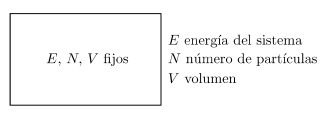
\includegraphics[width=0.4\textwidth]{microcanonico.png}
  \end{center}
\end{figure}

\subsection{Ensamble canínico }
$ T,N,V  $ fijos.Es usado para describir sistemas contenidos en un volumen $ V  $ que se encuentra en contacto con un baño térmico a temperatura $ T  $.La energía interna $ U  $ corresponde al promedio estadístico de la energía en el ensamble $ U = <E>  $ es una cantidad que permanece constante cuando el sistema se encuentra en equilibrio.
\begin{figure}[H]
  \begin{center}
    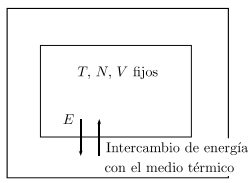
\includegraphics[width=0.25\textwidth]{canonico.png}
  \end{center}
\end{figure}
\subsection{Ensamble grancanónico }
Usado para describir sistemas abiertos contenido en un volumen $ V  $, que se encuentra contenido en un baño termico a temperatura $ T  $ y con un baño de partículas. La energia interna $ U  =<E>$ y el numero de particulas $ N  $ corresponde al promedio del numero de partículas en el ensamble $ N = <N>  $ y son cantidades que permanecen constantes cuando el sistema se encuentra en equilibrio termodinamico.
\begin{figure}[H]
  \begin{center}
    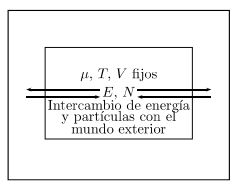
\includegraphics[width=0.25\textwidth]{grancanonico.png}
  \end{center}
\end{figure}

\section{Operador matriz densidad de probabilidad }
Se denota por $ \hat \rho  $. Hay que notar que un operador $ \hat{\mathcal A } $ queda definido cuando sus elementos matricuales son conocidos $ (\phi_l , \hat{\mathcal A }\phi_j) = \mathcal A _{lj } $.

Usando otra base de estados $ \{\ket{\phi_j' }\} $ pueden ser determinados por 
\begin{gather*}
  (\phi_l', \hat{\mathcal A }'\phi_j' ) = \mathcal A' _{lj }  
\end{gather*}
donde 
\begin{gather*}
  \hat{\mathcal A'} = \hat S \hat{\mathcal A} \hat S ^ {-1 }   
\end{gather*}

\hfill 

\hfill 

\hfill 

Definimos $ \rho _{lj }  $
\begin{gather*}
  \rho _{lj } = \bra{\phi _l }\hat \rho\ket{\phi_j } = (\phi_l, \hat \rho \phi_j ) \equiv \delta _{lj } \left|b_j \right| ^2   
\end{gather*}

\section{Postulado fundamental desde la perspectiva cuantica }
Tenemos 
\begin{gather*}
  \displaystyle\sum_{j }^{} \left|b_j \right| ^2 = \displaystyle\sum_{j }^{} \delta _{jj } \left|b_j \right| ^2 
\end{gather*}
y 
\begin{gather*}
  \rho _{jj }  \equiv (\phi_j , \hat \rho \phi_j ) = \delta _{jj } \left|b_j \right| ^2
\end{gather*}
Por lo tanto 
\begin{gather*}
  \displaystyle\sum_{j }^{} \left|b_j \right| ^2 = \displaystyle\sum_{j }^{} (\phi_j, \hat \rho \phi_j ) 
\end{gather*}
Partiendo de la igualdad podemos llegar a
\begin{gather*}
  \displaystyle\sum_{j }^{}\left|b_j \right| ^2(\phi_j, \hat{\mathcal A } \phi_j ) = \displaystyle\sum_{j }^{} (\phi_j, \hat \rho \hat{\mathcal A } \phi_j ) 
\end{gather*}


\end{document}
